\documentclass[10pt,a4paper]{article}
% \documentclass[a4paper,
% 10pt,
% DIV 10]{scrartcl}

\usepackage[utf8x]{inputenc}
\usepackage[english]{babel}
\usepackage{amssymb}
\usepackage{amsmath}
\usepackage{amsmath}
\usepackage{url}
\usepackage{graphicx}
\usepackage{watermark}
\usepackage{xspace}
\usepackage{paralist}
\usepackage{xargs}
\usepackage{research}

\addtolength{\textheight}{-2cm}
\addtolength{\textwidth}{2cm}
\addtolength{\textheight}{4cm}
\addtolength{\oddsidemargin}{-12mm}


\pagestyle{empty}

\begin{document}
\watermark{\put(-95,-760){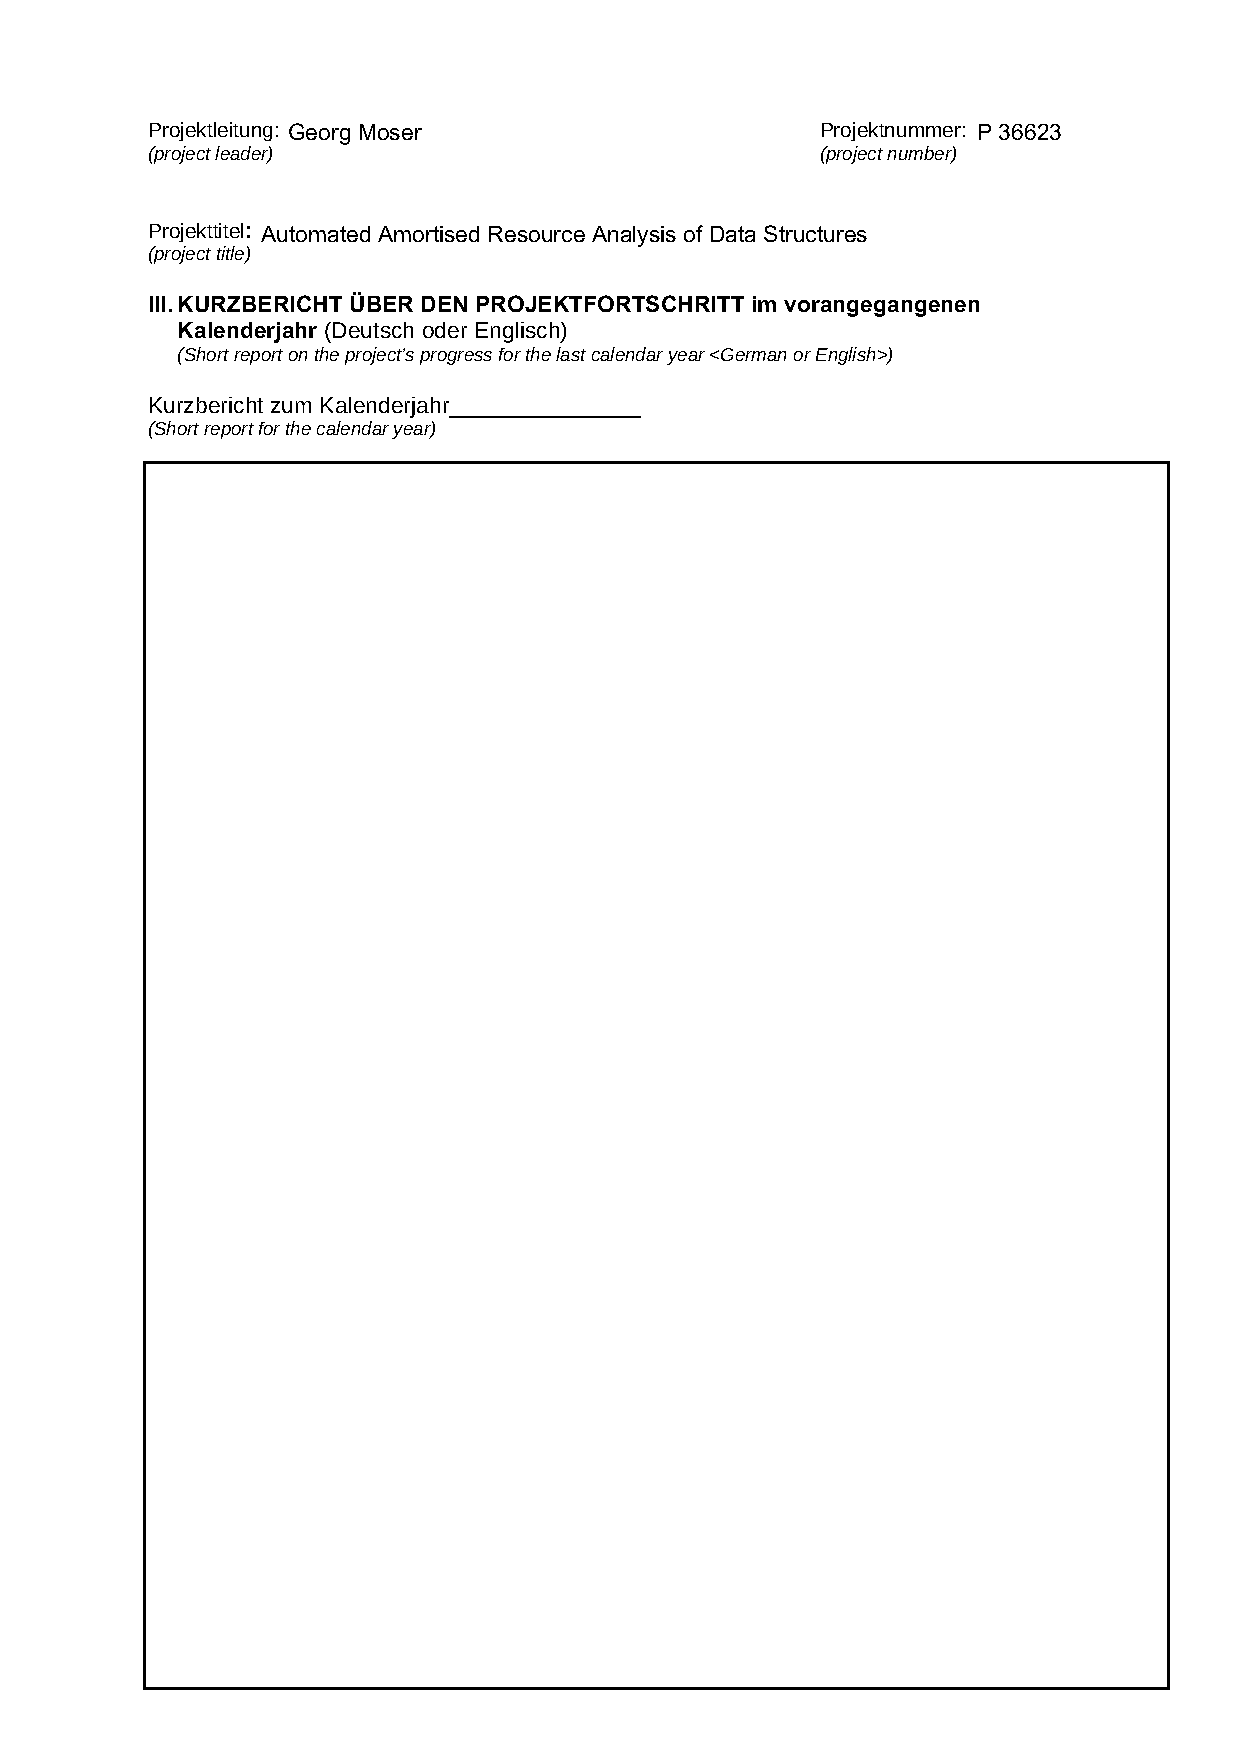
\includegraphics{template.pdf}}}

\vspace*{23mm}
\noindent\hspace{35ex}
2025

\vspace*{10mm}

\begin{center}
\large \normalsize Progress Report AUTOSARD 
\end{center}

During the last project year, we have taken next steps towards Work Package~1--3 and
continueed our formalisation efforts.

As reported last year, we have obtained a generalisation of the type system underlying our prototype~\atlas,
as well as a re-implementation of our prototype implementation. This generalisation led to the
automated amortised complexity analysis of novel data structures, namely \emph{skew heaps},
\emph{weight-biased leftist heaps} and \emph{rank-biased leftist heaps}.

These data structures
constitute challenging case studies for our automated analysis and we are confident that the
added theoretical and practical functionalities significantly widen the scope of such an
analysis, for example to standard data structures like \emph{AVL trees}. We note that \emph{skew heaps} have
been considered a challenge to our efforts in our last project meeting, as reported. These investigations
have already be accepted for publication~\cite{WMSZ26}. A comprised version of these investigations
will be suspect to a journal version, which is in preparation.

With respect to the formalisation of data structures, we have continued our recent efforts 
on the formalisation of \emph{zip trees}, a probabilistic data structure developed
by Robert Tarjan, Caleb Levy and Stephen Timmel~\cite{TarjanLT19}. Zip trees are isomorphic copies to
\emph{skip lists} introduced in 1990 by William Pugh.
%
Our formalisation has been developed in Liquid Haskell.
(Liquid Haskell is an interactive theorem prover, build on top of the functional
language \Haskell.)

Further, we started working on Work Package~2. For further publication within the project, see~\cite{FrontullMM25,SchneckenreitherM25}.

Finally, to improve dissemination of AUTOSARD's results, we again hosted a workshop at the University Centre Obergurgl. Apart from project participants, we were joined by Bob Atkey, from the University of Strathclyde, UK and Anton Lorenzen, from the University of Edinburgh. Among other talks, Atkey gave an inspiring tutorial on advanced type systems and Lorenzen presented his works on persistent data structures, results
that are pertinent to the project's Workpackage~2.

\bibliographystyle{plain}
\selectlanguage{english}
\small
\bibliography{references}

\end{document}
